\chapter{A New Approach}

In this chapter, we will present a novel approach for rendering a scene with dynamic light source efficiently. This method is based d on the standard GPU-based photon mapping rendering system, using an augmented kd-tree data structure and localized updating algorithm for rendering.  

In the first 2 sections of this chapter, We will have an overview on our approach and comprehensive description of the data structure that we use and related algorithms. Then we will look at some of the GPU implementation details. 

\section{Overview} 

As described in chapter 2, we build a global kd-tree as the photon map for irradiance estimation. However, the global photon map is rebuilt from scratch every frame, this process is time consuming due to the complexity of kd-tree building algorithm on GPUs and can be avoided. 

Instead of building a global kd-tree for photons, we re-use the same kd-tree for the geometry objects(triangles) which is static and associate the geometry and the photons data for efficient KNN search and update for dynamic scene. 

For each frame, the photons are shot from the light source and stored in an array, then we build the kd-tree for the geometry objects if it is required, for the scenes that don't include animated objects we will skip this process. Given the photons data in the scene and the built kd-tree for geometry, we build our data structure, compress the memory bind it to the texture memory for a better memory accessing performance. In rendering phase, instead of using photon map for radiance estimation, we use the kd-tree and our photon queue perform KNN search. Further details of the data structure will be presented in the following section. 

The update process of photons queue is straightforward. It depends on the photon data from the previous frames. Here we keep track of all the photons data of a range of frames with a pair of indices, the indices can be updated and maintained efficiently. Further details will be presented in following section.  

\section{Data Structure and Algorithm} 

\subsection{Data Structure}

\begin{figure}[htp] 
    \centering 
    \fbox{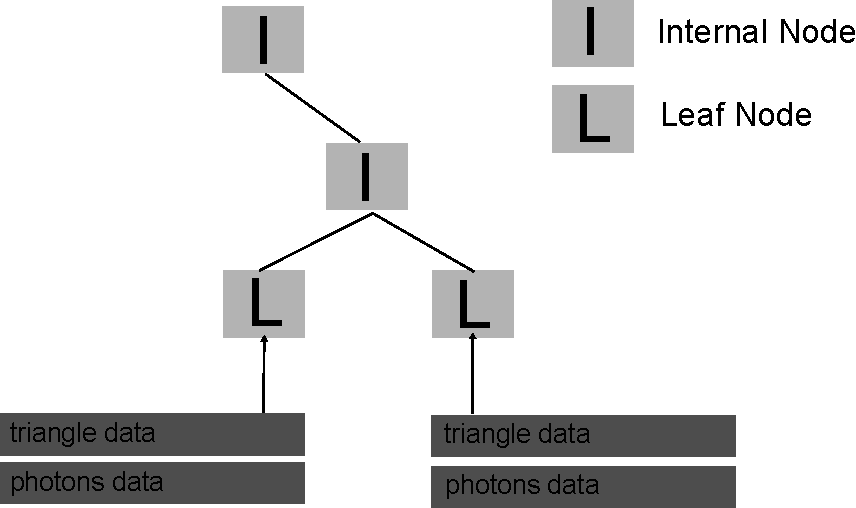
\includegraphics{imgs/kd_leaf_photons.pdf}}
    \renewcommand{\thefigure}{\thechapter.\arabic{figure}}
    \caption[]{Radiant flux from a point light source is passing through the spheres around the light.}
    \label{fig:kd_leaf_photons} 
\end{figure}  

As shown in figure \ref{fig:kd_leaf_photons}, in addition to the triangle data, the photons data in the scene is also logically associated with the leaf nodes of the kd-tree. As the kd-tree for the scene actually encodes the spatial relationship among the geometry, and the photons will be stored when they hit the objects with diffuse objects, we attach the photons fall into the spatial region occupied by the bounding box of a kd-tree leaf node. 

\begin{figure}[htp] 
    \centering 
    \fbox{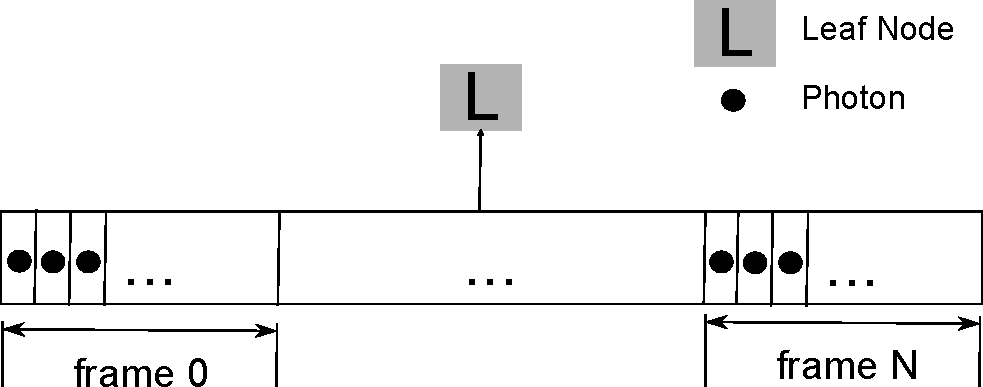
\includegraphics[width=\linewidth]{imgs/kd_leaf_photons_2.pdf}}
    \renewcommand{\thefigure}{\thechapter.\arabic{figure}}
    \caption[]{Radiant flux from a point light source is passing through the spheres around the light.}
    \label{fig:kd_leaf_photons_2} 
\end{figure}  

In figure \ref{fig:kd_leaf_photons_2} we have a more detailed view on how the photons data organized. The photons shot to the scene in one frame of rendering are stored followed by the photons of next frame. When implementing this organization on GPU, all actual photons data (positions, incident directions and power) is stored in a seperate array, the indices of the photons associated with kd-tree leaf nodes are stored instead of the actual photon data. 

\subsection{Construction} 

Building the logical connection between photons and leaf nodes is simpler than build a global kd-tree for the photon map. Firstly, we found out the the leaf nodes from the built kd-tree in parallel. This can be done checking a flag set when building the kd-tree. Given the indices of leaf nodes, we can retrieve the bounding box from the small node list generated in kd-tree construction phase(see \ref{subsec:kdtree_construction}). Then we check which leaf node certain group of photons should fall into in parallel by performing fast point-box intersection testing. For each leaf node, the number of photons can be calculated with a parallel reduction operation. Further details on physical memory arrangement and implementation of the data structure  will be presented in section \ref{sec:impl_detials}. 

\subsection{Update} 

When a frame of image is rendered, new photons will be shot into the scene and be stored in the same global array with previous frames and for each leaf node, we need to keep track of the range of the photons that are active for rendering the next frame. For each leaf node, we maintain two pointers(indices), start and end index, indicating the range of the photons used for rendering. We move the end pointer forward as there are new photons coming, move the start pointer forward when there are some old photons we need to discard. We use a pre-defined threshold from count to determine how many frames of photons data we want to make active, we keep accumulating the photons every frame until we reach that threshold value. When the threshold frame count 
is reached, we move forward the start pointer to avoid there are too many photons than there should be. Since the number of photons per frame is known, the stride of moving start pointer can be calculated. However, in GPU implementation, the step in bytes used to increment the pointer is usually larger than the exact size of photons data we want to discard, since the memory will be padded when it is allocated for better memory accessing performance. Further details will be presented in section \ref{sec:impl_detials}. 

\subsection{Rendering} 

Rendering with our data structure does not differ much from the standard photon mapping rendering algorithm. In rendering phase, we cast the rays from the camera into the scene in parallel and perform KNN search using the kd-tree already built for the geometry, when we reach the leaf nodes we use our data structure to find the photons data for particular leaf node and gather the photons for radiance estimation. 

\section{Implementation Details} 
\label{sec:impl_detials} 

\subsection{Data Organization} 
\label{subsec:data_org}

\paragraph{KD-Tree Data} 

The kd-tree data should be carefully organized when implemented with CUDA to improve traversal performance. In \ref{subsec:kdtree_construction}, we have already described the kd-tree building algorithm introduced in \cite{Zhou2008}, but some of the details that are critical to the program's overall performance still need to be discussed here. 

The final node list generated when the kd-tree is built is not sufficient for fast traversal algorithm, it contains too much useless information and will hit the performance since it is not friendly to cache pre-fetch. Therefore we compress and re-organize the traversal related data of the kd-tree nodes to reduce the memory access. The entire kd-tree is stored in a structure of several contiguous arrays. The structure is defined as following:  

% Code Snippet
\lstinputlisting{kdtree_data_def.cpp} 

The traversal data is compressed into an unsigned integer array, as shown in the following figure: 

\begin{figure}[htp] 
    \centering 
    \fbox{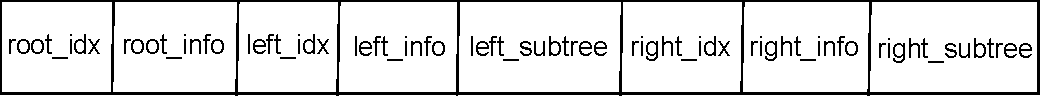
\includegraphics[width=\linewidth]{imgs/kdtree_data_memory_layout.pdf}}
    \renewcommand{\thefigure}{\thechapter.\arabic{figure}}
    \caption[]{Compacted kd-tree data memory layout.}
    \label{fig:kdtree_data_memory_layout} 
\end{figure}  

Where root\_info, left\_info and right\_info are the parent information for the root, left and right child node(if left and right node are inner nodes). This is a compressed form of what is needed during kd-tree traversal. Parent information stores two unsigned integers, hence two elements in the d\_preorder\_tree array. The first unsigned integer contains several information of the inner node: the split axis takes 2 most significant bits and address of right node in the d\_preorder\_tree array, which is 0 if it is a leaf node, take the rest bits. The second unsigned integer stores the split position(a float value stored as unsigned integer). The address of left child node is not stored explicitly as it can be computed by skipping the parent info(2 unsigned integers) from current node's address. The 2 bits for split axis can represent \(x\) axis if it is 0, \(y\) axis if it is 1 and \(z\) axis if it is 2. 

Where the root\_idx, left\_idx and right\_idx are the indices of the root, left and right nodes. The indices can be used to access the other arrays such as the node extents array. The type information of the nodes is also encoded in the indices, if it is a leaf node, the most significant bit(MSB) is set, else the MSB is not set, this improves leaf detection performance because it avoids reading child information. The above format applies only for inner nodes, for leafs, instead of parent information, element count and element indices are stored. The element indices are relative to the underlying triangle data. Hence we have the following format: 

\begin{figure}[htp] 
    \centering 
    \fbox{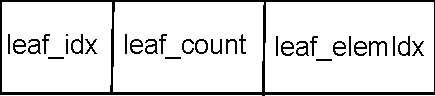
\includegraphics{imgs/kdtree_data_memory_layout_2.pdf}}
    \renewcommand{\thefigure}{\thechapter.\arabic{figure}}
    \caption[]{Compacted kd-tree data memory layout.}
    \label{fig:kdtree_data_memory_layout} 
\end{figure}  

\paragraph{Photons Data} 


\paragraph{Connection Between KD-Tree and Photons Data} 

The connection between KD-Tree leaf nodes and photons data is stored as a structure of several data array like storing other type of data on GPU side. 

\subsection{Algorithm Description} 

\subsubsection{Construction}  

\begin{spacing}{1.3} 

\begin{algorithm}[H]
	\SetAlgoLined
	\SetKwInOut{Input}{input}\SetKwInOut{Output}{output}
	\Input{KD-Tree Data} 
	\Input{Photons Data} 
	\Output{KD Leaf Nodes Photons List} 

	leafNodesMarks 	\(\leftarrow\) new array; \\
	leafNodesIndices 	\(\leftarrow\) new array; \\
	identityIndices 	\(\leftarrow\) (0, 1, 2 ... n); \\ 

	\For{All nodes of KD-Tree in parallel} {
		leafNodesMarks \(\leftarrow\) mark leaf nodes; \\
	}

	leafNodesIndices \( \leftarrow \) new array;	 \\
	tempArray \(\leftarrow\) \emph{Multiply} identityIndices and leafNodesMarks; \\
	leafNodesIndices \( \leftarrow \) \emph{Compact} tempArray; 
	 
	\For{All KD-Tree leaf nodes in parallel} {
		\For{All photons of current frmae in serial} {
			Perform point-box intersection detection. \\ 
			Store indices of photons 
		}
	}
	
	\For{All leaf nodes of KD-Tree in parallel} {
		\If{frame counter \(<\) max frames} {
			Store photons indices of current frame with current end pointer. 
		}

		Update start and end pointer for current leaf node.
	}
	
	\caption{Classify photons to kd-tree leafs. } 	
	\label{algo:build_kdleaf_photons} 
\end{algorithm}

\end{spacing}

\vspace{30pt}

In algorithm \ref{algo:build_kdleaf_photons}, it takes two major pieces of input data, the kd-tree data constructed for the scene and the photons data shot in the scene. The photons data is updated every frame by inserting new photons to an big chunk of buffer resides in GPU memory. Similar to the organization of underlying triangle data for kd-tree nodes, the memory for each frame of photons is aligned to a fixed size to enable coalesced memory access which may improve the performance considerably. This is one of the most important good practices for CUDA programming, because if the threads in a block are accessing consecutive memory locations, then all the accesses are combined into a single request by the hardware. However organizing data in this way will bring extra complexity for implementation because we have to keep track of the locations of beginning of next valid chunk of data for data accessing and there will be holes contained in the whole data array. Therefore move the pointer from \(i\)th frame to \(i+1\) frame requires increasing the pointer by maximum size of memory of \(i\)th frame which is aligned to a fixed size. 

We firstly mark the leaf nodes from the input kd-tree data, given the data definition described in the section \ref{subsec:data_org}, we only need to look at all the nodes and test if the MSB of the node's index is set. The indices of nodes can be retrieved from the kd-tree data. We store the result of marks in an array with the same number of elements as number of kd-tree nodes, the result will be 1 for a leaf node and 0 otherwise. The number of leaf nodes can be calculated by performing a data parallel reduction on this array. In order to store the indices of leaf nodes into an array of our data structure, we use another temporary local array and fill it with identity values \( (0, 1, 2 ... n-1) \), where \(n\) equals to the total count of kd-tree nodes, then we use the marks of leaf nodes as a filter to select the leaf nodes by performing an array multiplication for each elements on these two arrays, lastly we need a data parallel algorithm, compact, to remove all the invalid value(0s) from the result of previous step and store the result. 

Our goal is that connect photons with kd-tree leaf nodes so that we can easily find the photons according to the indices of leaf nodes. So we need to classify the photons into an array with the same order of the indices of leaf nodes. For example, the \(a\)th leaf node associates with a range of photons [i ... i + n]. Firstly, we launch a kernel program on all leaf nodes performing the intersection detections between the bounding box and point on all of photons, if the photon is contained in a certain leaf node, then we store the indices of photons. 

The data structure used to store photons for kd-tree leaf nodes works in the similar way to the circular buffer. We store number of frames of photons in a contiguous buffer. The start and end pointer(indices) indicate a range of frames of photons that is valid for rendering this frame. The start pointer points to the first photons of first active frame and the end pointer points to the first photon of the last active frame. We have a frame counter indicating the number of frames we have in the range, therefore we can detect if the buffer is full by compare the frame counter and max frames capacity. 


\subsubsection{Render} 

\begin{algorithm} 
	\SetAlgoLined
	\SetKwInOut{Input}{input}\SetKwInOut{Output}{output}
	\Input{Query Point} 
	\Input{Camera Rays}
	\Input{Query Radius} 
	\Input{Diffuse Colors}
	\Output{Radiance} 
	
	\For{All intersection points in parallel} {
		Retrive diffuse color at intersection point; \\
		Retrive the normal vector at intersection point; \\
		Flip the normal vector if it is needed; \\ 
		irradiance \(\leftarrow\) rangeSearch(intersectPoint); \\
		radiance \(\leftarrow\) colorDiffuse \( \cdot Pi^{-1} \cdot\) irradiance; \\ 	
	}
	\caption{Radiance estimation with kd-tree and photons queue.} 	
	\label{algo:render_kdleaf_photons} 
\end{algorithm}

Algorithm \ref{algo:render_kdleaf_photons} shows the main framework of estimating the radiance at a query point in parallel. Each CUDA thread works on one query point. The key part of this computation is performing KNN range search around the query point with the kd-tree and the photons queue as input. The KNN range search function sums up all the power(flux) of photons and output the irradiance by dividing the flux by the area of circle centered at the query with a predefined radiance. 

\begin{algorithm}
	\SetAlgoLined
	\SetKwInOut{Input}{input}\SetKwInOut{Output}{output} 
	\Input{Query point position} 
	\Input{Query radius} 
	\Input{KD-Tree Data} 
	\Input{Leaf nodes photons queue}
	\Output{Number of photons found}
	\Output{Irradianc}
	
	totalFlux \(\leftarrow\) 0; \\
	todoStack \(\leftarrow\) new\ Array[KD\_MAX\_HEIGHT]; \\
	nodeAddr \(\leftarrow\) 0; \\

	\While{\(nodeAddr >= 0\)} {

		idxNode \(\leftarrow\) kdTreeData.preorderTree[nodeAddr]; \\ 
		isLeaf \(\leftarrow\) idxNode\ \&\ 0x80000000; \\ 
		idxNode \(\leftarrow\) idxNode\ \&\ 0x7fffffff; \\ 
		
		\While{\(NOT\ isLeaf\)} {
			leftNodeAddr \(\leftarrow\) nodeAddr+1+2; \\
		
			parentInfo \(\leftarrow\) GetParentInfo(kdTreeData); \\
			splitAxis \(\leftarrow\) GetSplitAxis(parentInfo); \\ 
			splitPos \(\leftarrow\) GetSplitPos(parentInfo); \\
			rightNodeAddr \(\leftarrow\) GetRightNodeAddr(parentInfo); \\
		
			distSqr \(\leftarrow\) Sqr(queryPoint[splitAxis] \(-\) splitPos); \\ 
			
			nodeAddr \(\leftarrow\) leftNodeAddr; \\
			otherNodeAddr \(\leftarrow\) rightNodeAddr; \\
			\If{queryPoint[splitAxis] \(>\) splitPos} {
				nodeAddr \(\leftarrow\) rightNodeAddr; \\
				otherNodeAddr \(\leftarrow\) leftNodeAddr; \\
			}
			\If{ distSqr \(<\) queryDistSqr } { 
				todoStack[todoPos++] \(\leftarrow\) otherNodeAddr; \\ 
			} 
			
			Read node index + leaf info (MSB) for new node. \\
		}
		
		/* Now we have a leaf node */ \\
		photonIdx \(\leftarrow\) photonsQueue.start; \\
		numPhotons \(\leftarrow\) photonsQueue.numPhotons; \\
		\While {has more photons} {
			photonPos \(\leftarrow\) GetPhotonPos(photonIdx); \\
			pointDistSqr \(\leftarrow\) ComputeDistantSqr(queryPoint, photonPos); \\
			\If {pointDistSqr \(<\) queryDistSqr} {
				totoalFlux \(\leftarrow\) Add the flux of photons; \\
			} 
		} 
		\(nodeAddr\) \(\leftarrow\) Pop next node from next stack; \\	
	}	
	
	\Return irradiance \(\leftarrow\) totalFlux \/ maxRadiusSqr * Pi; \\ 
	
	\caption{Range search with kd-tree and photons queue.} 	
	\label{algo:knn_kdleaf_photons} 
\end{algorithm}

In algorithm \ref{algo:knn_kdleaf_photons}, we present the KNN range search using our data structure. The basic layout of the algorithm follows the standard while-while iterative traversal scheme.  We first allocate an array as the stack for the kd-tree traversal. Note that this array resides on the local memory of the CUDA thread running this algorithm, therefor the access to local array is always coalesced. Then we visit the kd-tree nodes in pre-order style using the compressed kd-tree data. If the current node is an internal, then we determine which subtree we will go deeper by compare the position of query point and split plane with respect to the split axis. If the other child node is in the range of search radius, it is going to be pushed to the stack. When a leaf node is reached, we look up the photons queue in which the range of photons for searching is marked by the start and end pointer and iterate over the photons finding the ones in the searching radius and calculate the irradiance. 

